\documentclass{beamer}
\usetheme{Singapore} % My favorite!
\setbeamercovered{invisible}
% To remove the navigation symbols from 
% the bottom of slides%
\setbeamertemplate{navigation symbols}{} 
%
\usepackage{algpseudocode}
\usepackage{verbatim}
\usepackage{algorithm}
\usepackage{tikz}
\usepackage{pgf}
\usepackage{xxcolor}
\usetikzlibrary{arrows,shadows,petri}
%                              wg. tokens
\usepackage{verbatim}
\usepackage{graphicx}
%\usepackage{bm}         % For typesetting bold math (not \mathbold)
%\logo{\includegraphics[height=0.6cm]{yourlogo.eps}}
%
\title[Short title of the talk]{Network Based Modeling for the Spread of Scientific Ideas }
\author{Mayra Berm\'udez, Sara Grimm \& Rzgar Hosseini}
\institute[U of X]
{ ETH Zurich \\
\medskip
%{\emph{email@domain.ca}}
}
\date{\today}
% \today will show current date. 
% Alternatively, you can specify a date.
%

\listfiles
\begin{document}
%
\begin{frame}
\titlepage
\end{frame}
%
\begin{frame}
\tableofcontents[pausesections]
\end{frame}

%









\section{Spread of scientific ideas}
\begin{frame}
{Spread of scientific ideas}
\begin{figure}
[htp]
\begin{center}
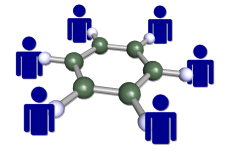
\includegraphics{science_network_150}
\end{center}
\label {fig1}
\end{figure}
\end{frame}
%
\begin{frame}
In this slide I' would like to add a figure very similar to the last one but with some labels and different color in the nodes. A draft of it is the Figure1beamer. I haven't manage to put here! Hopefully I'll do it later!
\end{frame}
%
\section {Introduction and Motivations}
\begin{frame}
\frametitle{Introduction and Motivations}
\begin{itemize}
\item But how do ideas spread? \pause
\item Research has shown that not only does the nature of information or innovation influence the diffusion of it, but also that the structure of a network influences the diffusion dynamics. \pause
\end{itemize}
\end{frame}
%
\begin{frame}
\begin{itemize}
\item Here, we try to simulate the spread of scientific ideas in different networks. \pause
\item The model presented is based on two studies: one that investigated critical parameter values for complex contagion and another that investigated critical values of a rewiring parameter.\pause
\end{itemize}
\end{frame}
%
\begin{frame}
{Fundamental Questions}
The main goals of this simulation study are to investigate how network structure influences the distribution of ideas, and how the distribution of ideas influences network structure.
\end{frame}
%
\begin{frame}
{Some terminology}
\alert {I'll do a link to this slide, in this way we can go back to this slide every time that be necessary. I'll do that the table fix here, but I'm not sure what do you think if this information should be in a table? or in other way?}
\begin{table}[ht]
\caption{List of terminology} % title of Table
\centering % used for centering table
\begin{tabular}{c c c c } % centered columns (4 columns)
\hline\hline %inserts double horizontal lines
 & Term\\ [0.5ex] % inserts table
%heading
\hline % inserts single horizontal line
Neighborhood index & The fraction of the holders of the same idea\\
\,&  who are neighbor as well averaged over all ideas.\\
\hline
Intra-idea distance& The average distance between \\
&holders of the same idea in the network.\\
\hline
Dominant frequency & The frequency of the dominant idea\\
& in the network at each time steps of the
simulation.\\
\hline
Average dominance time& The average number of time steps \\
&in which the dominant idea keeps its
dominance.\\
\hline
Novelty index& The fraction of newly generated ideas.\\
\hline
Average shortest path & The average number of steps\\
& along the shortest paths for all possible pairs of network nodes.\\
\hline
Clustering coefficient &  A measure of degree to which\\
& nodes in a graph tend to cluster together.\\
\hline
Degree of connectivity &  The number of edges incident to the vertex.\\
\hline
Connected component & A subgraph in which any two vertices are\\
 &connected to each other by paths, and which is connected to no\\
  &additional vertices in the supergraph.\\
\hline
Diameter of network& The longest of all the calculated shortest paths\\
& in a network.\\
\\ [1ex] % [1ex] adds vertical space
\hline %inserts single line
\end{tabular}
\label{Tab2} % is used to refer this table in the text
\end{table}


\end{frame}
%
\begin{frame}
During the study we vary :
\textbf{Parameters}
\begin{itemize}
\item Probability of rewiring $\phi$
\item Rate of innovation $\alpha$
\item Complex contagion threshold  $\delta$ respectively) 
\end{itemize}
\textbf{Network structures}
\begin{itemize}
\item Random
\item Scale free
\item Small world
\item Caveman
\end{itemize}
\textbf{Idea distributions}
\end{frame}
%
\begin{frame}
{Before simulations: our thoughts}
{Effects of Network Structure on Idea Distribution}
\begin{itemize}
\item Given a starting network and a random idea distribution, how do different network structures (see Section ) affect the distance between nodes that have the same idea (intra-idea distance)? 
\item How do they affect the neighbourhood index? 
\item How do they change the emergence of dominant ideas and their time of dominance? How do their effects depend on the values of $\phi$, $\alpha$ and $\delta$?
\end{itemize}
\end{frame}
%
\begin{frame}
%\subsubsection
{Effects of Idea Distribution on Network Structure}
Given a starting idea distribution and a caveman network structure, how do different idea distributions affect the average path length and diameter of the network? Do they change the number of connected components in the network? Do clusters form differently, and how does the clustering coefficient change? What does the distribution of node degree looks like? How do these effects depend on the values of $\phi$, $\alpha$, and $\delta$?
-random\\
-paralell\\
-nonparalell\\
\end{frame}
%
\begin{frame}
\frametitle{Description of the Model}

The model used here is based on a study by %\citet*{HN2006}. 
  Each simulation begins with a specified network structure as well as a distribution of the `idea' (or state) of the nodes. At each time step a node either changes its idea to that of one of its neighbours' ideas if its frequency surpasses a defined threshold, rewires to connect with a node that has the same idea, or generates a novel idea (this is the innovation parameter). 
\end{frame}
%
\begin{frame}
Given the network structure and node states, three parameters are introduced: $\phi$ (probability of rewiring), $\alpha$ (probability of innovation), and $\delta$ (complex contagion threshold). As in \alert {cite{HN2006}}, $\phi$ is a value from zero to one, and is the probability that one of the edges of a randomly chosen node \emph{i} will be changed to connect to another node \emph{j} that \emph{i} is unconnected with. We decided to add one more criterion to this definition: node \emph{j} is a node that has the same idea as node \emph{i}. This encourages the simulations to reflect a common tendency of individuals to seek out others who think like them. If there is no such node \emph{j}, then the chosen node will do nothing.
\end{frame}
\begin{frame}

At each time step a node may `come up with a new idea' with a probability of $\alpha$. This value is small to reflect that novel ideas are not frequently observed.


We introduced a node threshold $\delta$ to the general model in order to investigate the behaviour of complex contagion as opposed to simple contagion. This was motivated by a study by \alert{citet*{CM2007}}. Simple contagion is well suited for modeling the spread of diseases since they may often be passed on by a single contact with an infected individual. However, as our intuition may suggest, other kinds of innovations raise questions about the legitimacy and credibility of the innovations themselves, and may thus require exposure to multiple sources of the innovation. This is called complex contagion. Models usually represent it in two ways regarding the number of connected sources that must have adopted an innovation in order to influence the agent (or individual) in question: it is either a fixed number (greater than one) or a fraction (between zero and one, inclusive). Our simulation used the second formulation since the degree of individual nodes varied across network structures.
\end{frame}
%
\begin{frame}
%\subsection
{Networks}

For the purposes of our simulations, we used four network structures. These structures can be characterized by properties such as average shortest path lengths, clustering coefficients, and the degree of connectivity (see Table \ref{Tab2} for definitions). Below are short descriptions of each network structure. In order to compare between different structures, the network structure parameters were chosen such that the mean degree of the networks were similar (approximately 25). For further details about parameter values, see Table \ref{Tab1}\\
free scale\\
caveman\\
random\\
smallworld\\
%\subsection
{Ideas}
\end{frame}
%
\begin{frame}
\frametitle{Implementation}
Our simulation comprises mainly two parts: the phase 1 corresponding to the study  of the effect of network structure on the idea distribution, and phase 2 where we study how the distribution of the ideas affect the topology of the network. These two phases are implemented in the same MATLAB file \textbf{mainscript.m}. Implementation of both phases is divided into three steps. 
\\

\noindent \textbf{Step 1:} Network structure is chosen and we generate the adjacency matrix corresponding to that structure. The initial idea distribution is also generated.\\
\textbf{Step 2:} The updating process is done onto the chosen network structure.\\
\textbf{Step 3:} At this step a series of functions are called to get the results.
\end{frame}
%
\begin{frame}
%\subsection
{Step 1: Generating network structures and initial idea distribution}
%\subsection
{Step 2: Update}                
\alert{Here it suppose to be the algorithm}

\end{frame}
%
\begin{frame}
{Step 3: Getting results}

In the phase 1 we want to observe the influence of a certain network structure  on the distribution of ideas after the updating process (step 2). For this, it is necessary to search for features that reflect the final distribution of ideas. In this study we observed the following features:

\alert{??}

\end{frame}
%
\begin{frame}
{Discussion}

As previously mentioned, we observed that some features of the idea distribution varied with the type of network structure. We also observed that some features of the network structure varied with the kind of idea distribution implemented. Some of these results were intuitive and expected, while others were not.

Network structure mainly influenced two features of the idea distribution: the intra-idea distance and the neighbourhood index. The intra-idea distance was larger for the caveman and small world networks, as anticipated. However, contrary to expectations, the neighbourhood index was larger for these two structures, and the caveman structure did not decrease the frequency of dominance (and neither did any other structure).  Additionally, the values of $\phi$ and $\delta$ did correlate with changes in the values of the intra-idea distance (by decreasing it) and the neighbourhood index (with different effects depending on the structure), but not always: $\delta$ did not vary the results of the intra-idea distance or the neighbourhood index of the random and scale-free networks, and $\phi$ did not vary the neighbourhood index in the small world network. Lastly, and also contrary to expectations, increasing the $\alpha$ values increased the neighbourhood index of networks.


Four of the five features of the network structure changed with different idea distributions. The connected component interestingly remained one, regardless of the idea distribution and parameter values. Feature values of the anti-parallel and random idea distributions differed from those of the parallel distribution. Most features changed as expected: the clustering coefficient, average path length, and network diameter were larger when the parallel idea distribution was used as compared to the other two, and their values were similar to those of a caveman network structure. The clustering coefficient of the anti-parallel idea distribution networks did decrease, as expected. The degree distribution did increase in variance (becoming more similar to a normal distribution) for the networks that were initiated with a random or anti-parallel idea distribution, but the degree distribution of the parallel idea distribution networks resembled that of a scale-free power law. Values of $\phi$ influenced the features of the random and antiparallel distribution networks the most. However, the structure features of the networks with the random idea distribution were not more sensitive to parameter values as would have been expected; they behaved similar to those of the networks with the anti-parallel idea distribution. Values of $\delta$ only correlated with changes in the clustering coefficient of the networks with a parallel idea distribution, and only weakly. Values of $\alpha$ did not correlated with any changes of feature values. 
\end{frame}
%
\begin{frame}
\frametitle{Summary and Outlook}
To conclude our simulation study, our results support the general idea that network structure and qualities of the ideas held in them may mutually influence each other. The more rigid the structure of a network was, the more likely that the intra-idea distance and neighbourhood index of the network was larger. These two features varied more with the innovation rate $\alpha$ for less structured networks, and varied more with the complex contagion threhold $\delta$ for the most rigid structure - the caveman network. The average dominance time seemed to vary more with parameter values ($\phi$, $\delta$, and $\alpha$) than with the network structures, whereas the frequency of dominance of ideas did not decrease on average in the long run with any network structure.

A network in which the pattern of ideas held by the nodes are `in accord' within the clusters of the caveman network maintained more of the structure features of a caveman network. These values varied with values of rewiring probabilities $\phi$ and complex contagion threholds $\delta$. Networks with a random pattern of ideas or with a pattern with more `disaccord' within the clusters resulted in a structure that began to resemble a random graph more than a caveman network. These networks' values varied more with the parameter $\phi$ of rewiring. Nodes given the chance to rewire with nodes that share the same idea had more opportunity to do so in the random and `disaccord' idea patterns than in the pattern which already had much accord.

Thus, in addition to the structure of networks and the pattern of ideas in them, complex contagion thresholds, innovation rates, and the probability of creating new connections (while reflecting `preferences' of being connected with like-minded others) tend to influence features of the network. Several extensions to the proposed model could be investigated to better understand the relationships between network structure and idea distribution.
\end{frame}
%
\begin{frame}
paragraph{Rewiring criteria}
Future simulations may compare the emerging features of idea distributions not just between network structures, but also between different rewiring criteria. It is not clear how much of the features of the idea distribution in this simulation study was a result of the network structure or of the `preference' that nodes had in rewiring to like-minded nodes. Therefore, these results could be compared to (1) random rewiring or, to allow structure to play a larger role, (2) to allow random rewiring to nodes that are at most a distance of three nodes away. This is somewhat more realistic since most people connect with individuals who are somewhat in their vicinity through mutual connections. 

paragraph{Complex contagion and innovation}
Considering complex contagion, novel ideas in our model were at a disadvantage for spreading in the network. Allowing novel ideas to have a larger influence weight may be one way to grant the ability of them to spread to other nodes. Alternatively, the complex contagion threshold for novel ideas may be lowered.

paragraph{Random idea adoption}
Future simulations may investigate the effects of network structure on idea distributions by comparing to a `benchmark' model. This model would update the ideas of nodes at random, and thus the effects of connections may be better observed within network structures and then compared between network structures.
\end{frame}






\end{document}